\documentclass{OM_style}

\usepackage{enumitem}
\usepackage{graphicx}
\graphicspath{ {./Dokumentacija/} }

%ovdje dodate pakete ukoliko Vam neki treba

% ne dirati
\makeatletter
\DeclareOldFontCommand{\rm}{\normalfont\rmfamily}{\mathrm}
\DeclareOldFontCommand{\sf}{\normalfont\sffamily}{\mathsf}
\DeclareOldFontCommand{\tt}{\normalfont\ttfamily}{\mathtt}
\DeclareOldFontCommand{\bf}{\normalfont\bfseries}{\mathbf}
\DeclareOldFontCommand{\it}{\normalfont\itshape}{\mathit}
\DeclareOldFontCommand{\sl}{\normalfont\slshape}{\@nomath\sl}
\DeclareOldFontCommand{\sc}{\normalfont\scshape}{\@nomath\sc}
\makeatother

\newcommand{\CourseName}{I046 Moderni sustavi baze podataka}
\newcommand{\CourseURL}{www.mathos.unios.hr/index.php/607}
\newcommand{\Lecturer}{Slobodan Jelić}
\newcommand{\ScribeName}{Ena Pribisalić}
\newcommand{\LectureName}{Seminarski rad}
%%%%%%%%%%%%%%%%%%%%%%%%

%ispod smijete mijenjati postavke
\newcommand{\LectureType}{Dario Zavišić} %ovdje mozete promijeniti broj zadace
\newcommand{\LectureDate}{18.05.2020.} %ovdje mozete promijeniti datum


\begin{document}
%stil za stranicu
\pagestyle{OM_lecture}

% vasi podaci
\chapter{Hrvatske željeznice} %ovdje unosite svoje ime i prezime

Tema ovog seminarskog rada je baza podataka za Hrvatske željeznice, tj. HŽ Putnički prijevoz. Radi jednostavnosti ću Hrvatske željeznice oslovljavati s HŽ. Kako bi došli do konačnog modela baze podataka za HŽ, trebamo prvo razumjeti kako funkcionira takav sustav. Prilikom skiciranja modela entiteta i veza zamislio sam da bi se kupnje karata vršile ili online ili na stanici na blagajni. S obzirom na to, svaki kupac je registriran ili online ili ima svoju pametnu karticu. Shodno tome entitetu $KUPAC$ možemo pridružiti atribute kao što su njegov identifikacijski broj, njegovo ime, prezime, datum rođenja, adresa stanovanja, telefonski broj te razinu $popusta$ koju ostvaruje $KUPAC$. Njegov identifikacijski broj ćemo učiniti njegovim primarnim ključem kako bismo ga mogli kasnije lakše i efikasnije referencirati negdje. Sve njegove atribute postavimo da su obavezni prilikom popunjavanja njegove tablice. Kako znamo da HŽ nudi razne skupine $popusta$ s obzirom na status $KUPCA$, napravio sam da mi popusti budu zasebni entitet $POPUST$. U entitetu $POPUST$ sam definirao primarnim ključem atribut $popust\_id$ u kojem se id-ovi sastoje od riječi npr. 'student', 'umirovljenik' i sl. $popust\_id$ nam se time odnosi na status kupca i njegovu razinu prava na popust. Također sam definirao atribut $postotak$ koji odgovara određenom iznosu popusta za neku vrstu statusa. Oba atributa su mi obavezna prilikom popunjavanja tablice. Zatim entitet $KUPAC$ sam povezao s etitetom $POPUST$ na način da sam atribut $popust\_id$ u $KUPCU$ postavio da je strani ključ koji se odnosi na $popust\_id$ u $POPUSTU$. Pri čemu pupust mora imati jedan ili više kupaca, a jedan kupac mora imati samo jedan popust.

\phantom{................} 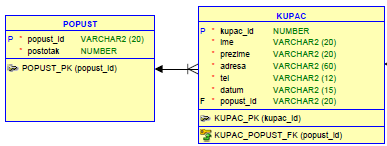
\includegraphics{popustkupac} \\

Time smo definirali sve što se tiče kupca i njegovog popusta, pa odlučujem napraviti entitet $POSTAJA$ u kojem ću definirati primarnim ključem atribut $postaja\_id$ i atribut $naselje$ koji mi se odnosi na imena gradova i općina u Hrvatskoj. Nakon definiranja entiteta $POSTAJA$ definiram entitet $VLAK$ u kojem mi je primarni ključ $vlak\_id$ i svakom vlaku još pridružujem dva atribuda koji su tipa bool, $brzi$ i $putnicki$ kako bi znali vrstu vlaka. Ovom entitetu nisam dodavao atribut $teretni$, jer mi se uglavnom baza bazira na kartama i kupcima, a teretni vlakovi ne prevoze ljude, osim strojovođe. Nakon što sam definirao entitete $POSTAJA$ i $VLAK$ smislio sam entitet koji bi mi služio poput informacija u kojem bi imao ID nekog putovanja, koji ima svoje polazište, odredište, cijenu, trajanje putovanja i ID vlaka koji vozi to putovanje. Tako sam napravio entitet $INFO$ koji ima primarni ključ $info\_id$ , atribute $polaziste$ i $odrediste$ na koje sam stavio strani ključ koji se odnosi na $postaja\_id$ u entitetu $POSTAJA$. Također sam definirao atribut $cijena$, $trajanje$ i $vlak\_id$ koji je strani ključ dobiven iz entiteta $VLAK$ i njegovog primarnog ključa $vlak\_id$. Veza između informacija i vlakova je takva da jedan vlak mora imati jedan ili više informacija, te jedna informacija mora imati jedan vlak. Veza između postaja i informacija je da jedna postaja mora imati jednu ili više informacija, a jedna informacija jednu ili više postaja. Izgled modela navedena tri entiteta možemo viditi na slici: \\

\phantom{...........} 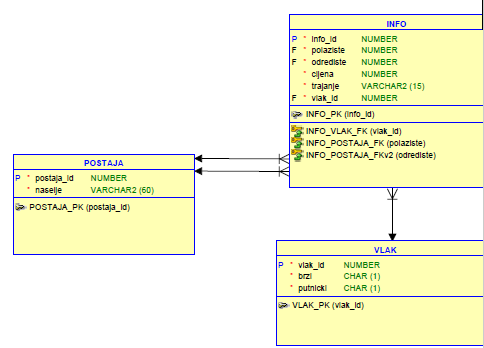
\includegraphics{postinfovlak} \\

Zatim kako bi došli do karata, ako bi kartu kupovali na blagajni, moramo imati i zaposlenika koji obavlja taj posao, ali također kupili kartu online ili na blagajni, moramo imati konduktera koji će pregledati kartu u vlaku i samog strojovođu koji upravlja vlakom. S toga sam definirao entitet $ZAPOSLENIK$ u kojem sam svakom zaposleniku dao njegov $zap\_id$ koji je ujedno i primarni ključ, te njegovo ime, prezime, adresa, telefonski broj, datum rođenja, njegova plača i njegova uloga, odnosno vrsta posla koju on obavlja u firmi. Kako bismo povezali određenog zaposlenika da radi na određenom mjestu kao što je npr. određeni blagajnik na određenoj postaji, tako i određeni kondukter i strojovođa u određenom vlaku. Definiram entitet $ULOGE$ u kojem mi primarni ključ čini strani ključ $zap\_id$ iz entiteta $ZAPOSLENIK$ i onda svakom zaposleniku pomoću stranih ključeva pridužujem atribute $uloge\_id$, $postaja\_id$ i $vlak\_id$. $uloge\_id$ ima 3 vrste id-a, 1 označava blagajnika/cu, 2 označava konduktera/icu, 3 označava strojovođu/icu, ako je $uloge\_id$ 1 znači da je blagajnik/ca u pitanju pa mu pridodajem na atribut $postaja\_id$ strani ključ koji dolazi iz neke postaje i time osigurava da mi na određenoj postaji može biti više blagajnika. Ako mi je $uloge\_id$ 2 ili 3 onda u atribut $vlak\_id$ pomoću stranog ključa pridužujem id vlaka u kojem radi kondukter ili strojovođa. Također time osiguravam da mi u jednom vlaku može raditi više konduktera i strojovođa. Jedan zaposlenik mora imati jednu ulogu, ali jedna uloga mora imati jednog ili više zaposlenika. Primjer modela pomoću slike: \\

\phantom{...........} 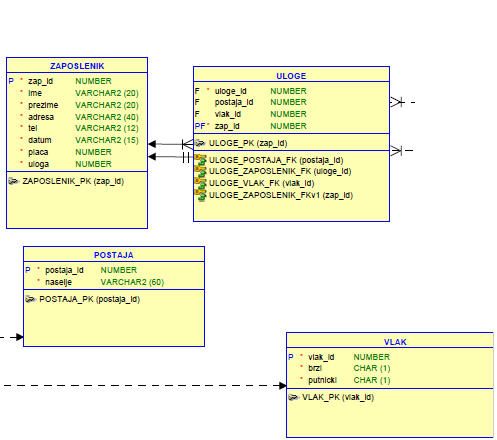
\includegraphics{zapuloga} \\


Sada kad imamo definirano entitete $KUPAC$, $POPUST$, $VLAK$, $POSTAJA$, $INFO$, $ZAPOSLENIK$ i $ULOGA$, možemo definirati i entitet same karte, odnosno $KARTA$. Znamo da nam svaka karta ili račun u trgovini imaju svoj broj, tako sam napravio i primarnim ključem atribut $karta\_id$. Svaka karta nam sadrži informacije poput polazišta i odredišta, zatim duljine trajanja putovanja, njegovu cijenu i vlak kojim se putuje, pa sam atribut $info\_id$ povezao stranim ključem koji dolazi iz entiteta $INFO$ s atributa $info\_id$. Zatim svaka karta ima svoj datum kupnje i informaciju vremena polaska vlaka, odnosno dodao sam atribute $datum$ i $vrijeme\_polaska$. Posljednje kako bi znali jel karta pripada osobi koja ju je kupila te je li na cijenu putovanja ide popust, dodao sam atribut $kupac\_id$ koji sam povezao pomoću stranog ključ koji dolazi iz entieta $KUPAC$ i njegovog atributa $kupac\_id$. Veza između kupca i karte nam kaže da kupac mora imati jednu ili više karata, a karta mora imati jednog kupca. Te da karta mora imati jednu informaciju i da jedna infomacija mora imati jednu ili više karata. Time smo dobili kompletan izgled modela entiteta i veza što možemo vidjeti na slici: \\

\phantom{............} 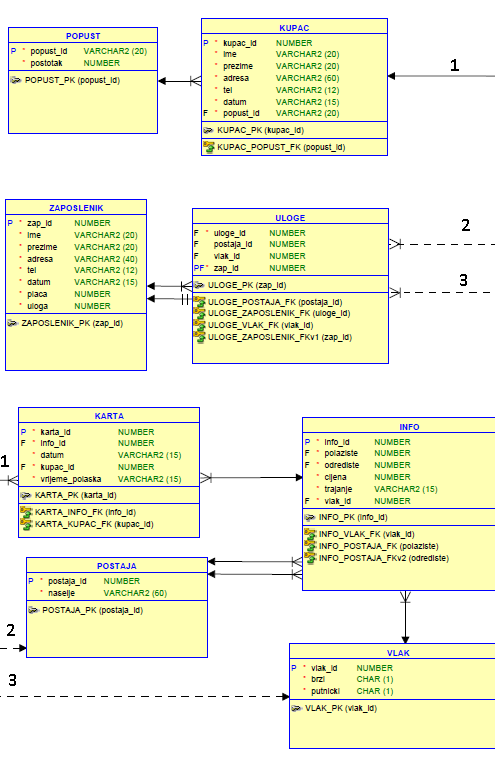
\includegraphics{fullmev} \\

Prilikom popunjavanja tablica koje sam kreirao u sql-u, počeo sam popunjavati prvo tablicu $POPUST$-i jer mi je ona potrebna kako bi popunio tablicu $KUPAC$. Primjer za INSERT kod popusta: \\
\\
INSERT INTO popust (popust\_id, postotak) VALUES ('student',50); \\
\\
U tablici $POPUST$ sam ubacio status 'nema' kao jedan od $popust\_id$-ova koji ima postotak 0\%, ako neka osoba nema ostvarena prava za neku skupinu. Zatim nakon popunjene tablice $POPUSTA$ popunio sam tablicu $KUPAC$ za koju sam INSERT operacije izgenerirao pomoću python skripte, primjer INSERT-a:\\
\\
INSERT INTO kupac (kupac\_id, ime, prezime, adresa, tel, datum, popust\_id) VALUES (1,'Luka','Horvat','Park Ivana Pavla II. 22','0992783282','26/10/1978','ucenik'); \\
\\
Nakon popunjenja tablice $KUPACA$, odlučio sam popuniti tablicu $ZAPOSLENIKA$ jer mi ništa drugo ne stoji na putu da bih morao prethodno popuniti prije njih. Također INSERT operacije za $ZAPOSLENIKE$ sam izgenerirao pomoću pythona, npr.:\\
\\
INSERT INTO zaposlenik (zap\_id, ime, prezime, adresa, tel, datum, placa, uloga) VALUES (1,'Marko','Bajić','Marusinac 2','0958231082','19/03/1981',10092,1);\\
\\
Prostaju mi još dvije tablice koje mogu popuniti bez ikakvih prethodno potrebno popunjenih tablica. Tablica $POSTAJA$ koja mi sadrži ID svake postaje te ime naselja, odnosno grada ili općine, sam isto izgenerirao pomoću pythona, gdje sam sav popis naselja čitao iz popisa od strane Ministarstva RH. Primjer jednog od 556 INSERT-a: \\
\\
INSERT INTO postaja (postaja\_id, naselje) VALUES (556, 'Zagreb'); \\
\\
Tablicu vlak nisam generirao nego ručno napisao s obzirom da nema puno atributa, a odlučio sam se da imam šest vlakova. Primjer INSERT-a: \\
\\
INSERT INTO vlak (vlak\_id, brzi, putnicki) VALUES (1,1,0); \\
\\
S obzirom da sam popunio tablicu $ZAPOSLENIK$ i tablice $POSTAJA$ i $VLAK$, sada mogu popuniti tablicu $ULOGE$, npr:\\
\\
INSERT INTO uloge (uloge\_id, postaja\_id, vlak\_id, zap\_id) VALUES (1,345,NULL,13);, \\
\\
gdje mi NULL vrijednost stoji ako zaposlenik ne radi na određenom mjestu.
Još mi preostaje popuniti dvije tablice pri ćemu je prioritet na tablici $INFO$, jer tablica $KARTA$ zahtjeva podatke iz tablice $INFO$.
Sve INSERT-e za tablicu $INFO$ sam isto generirao pomoću python skripte, primjer INSERT-a:\\
\\
INSERT INTO info (info\_id, polaziste, odrediste, cijena, trajanje, vlak\_id) VALUES (1,243,24,5895.89,'09:1:00',1); \\
\\
Konačno popunjavam tablicu $KARTA$ jer imam sve potrebno prethodno popunjeno, te za nju također koristim python skriptu, primjer INSERT-a:\\ 
\\
INSERT INTO karta (karta\_id, info\_id, datum, kupac\_id, vrijeme\_polaska) VALUES (1,246,'7/16/2020',1,'11:57:00'); 
\end{document}